\chapter{Ectopic Activation of the Spindle Assembly Checkpoint Signaling Cascade Reveals Its Biochemical Design}
\label{chpt:2}

\section{Building a semi-automatic data analysis pipeline to enable the processing of a large volume of data}
For mitotic duration assays requiring live-cell time-lapse imaging, we utilized a semi-automatic pipeline [implemented in MATLAB (MathWorks)] to facilitate data analysis \myref{DataAnalysisPipeline}. Images of fluorescence channel(s) were first pre-processed to remove backgrounds and corrected for shading. The background was obtained from a blank well containing only the imaging media. The shading pattern was calculated from a blank well containing the imaging media supplied with the corresponding purified fluorescence protein. Due to the lack of precise mechanical control of stage positioning on the IncuCyte\textsuperscript{\textregistered} ZOOM System (Sartorius) [but not so much on the ImageXpress\textsuperscript{\textregistered} Nano Automated Imaging System (Molecular Devices)], there is non-negligible jittering over time. Images of the phase-contrast transmitted light channel were registered (aligned) with the preceding image in the stack recursively (except for the first frame). The computed translations were then propagated to the calibrated fluorescence image stack(s).

Adherent mammalian cells typically assume a spherical shape from NEBD (nuclear envelop breakdown) to anaphase onset, while G\textsubscript{1}/S/G\textsubscript{2}/prophase cells usually assume a flattened shape on a plate. In slightly defocused phase-contrast transmitted light images, these cells appear as circles defined by high-contrast halo and shade-off artifacts \cite{PhaseContrastHalo}. Our semi-automatic pipeline utilized this to detect mitotic cells by convolving each image with kernels representing ``average'' mitotic cells (constructed by 2-D averaging of micrographs of manually picked mitotic cells of the same cell line). A threshold is then applied to the correlation matrix to convert it into a binary matrix. Connected components of high-correlation pixels (above a certain threshold of the pixel size) are recognized as mitotic cells. Centroids of these connected components were linked across successive frames to connect all frames of the same cell across the entire history from NEBD to anaphase onset (hereby defined as an ``event''). These events were then presented to the user in a graphical user interface (GUI), where the user can manually examine them carefully to either abandon a false event or to correct the frame index of NEBD/anaphase onset if necessary. The duration of mitosis is then calculated and corresponding $(x, y, t)$ coordinates are propagated to the fluorescence channel(s) to measure the fluorescence signal(s) of the cell.

\begin{figure}
    \centering
    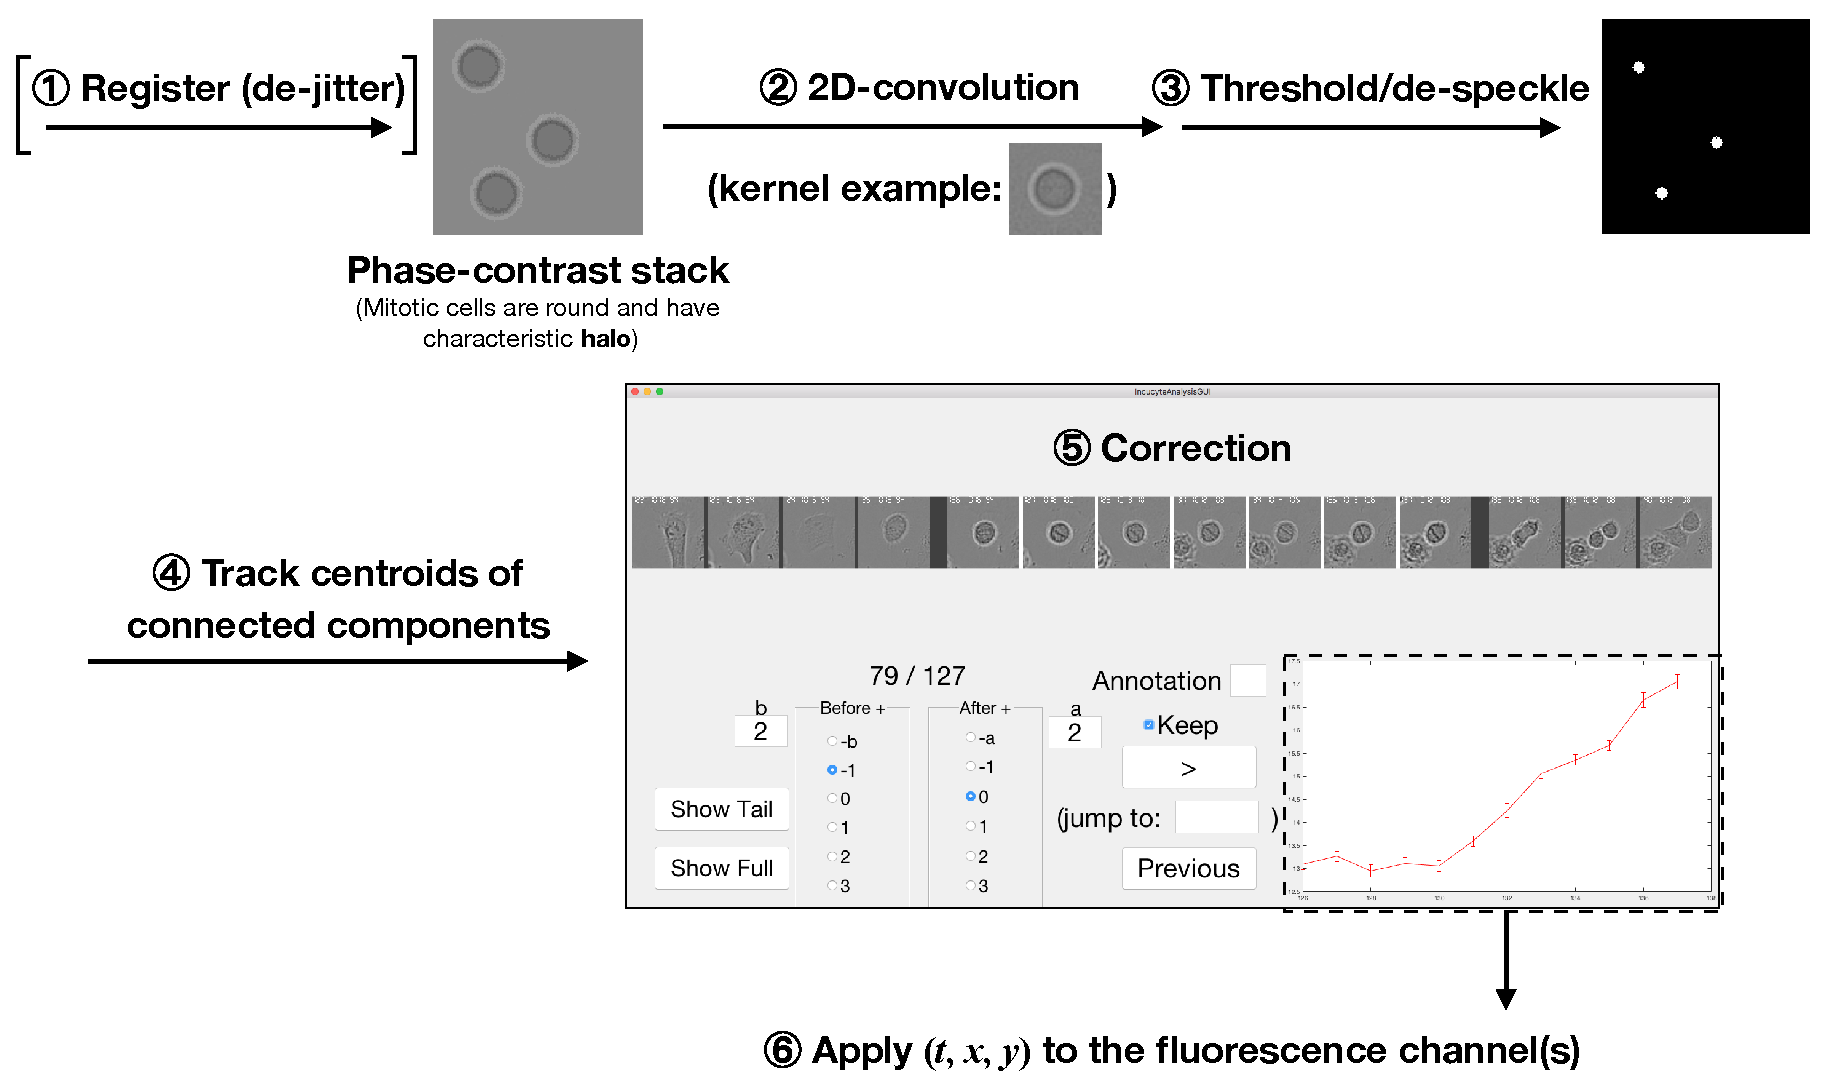
\includegraphics[width=0.95\textwidth]{chapters/figures/DataAnalysisPipeline.pdf}
    \caption{\textbf{A diagram illustrating the semi-automatic data analysis pipeline for mitotic duration assays.}}
    \label{DataAnalysisPipeline}
\end{figure}

\section{The distance between MELT motifs has a minor impact on the SAC activity}
\label{sec:examplesec3}
There are two major differences between the M1, M3, and M6 (M3-M3) eSAC constructs in the previous section: (1) that the total number of MELT motifs in the signaling scaffold are different and (2) the lengths of these signaling scaffolds are different. Even though the phosphodomain of \protein{Knl1} is largely unstructured and flexible \cite{UnstructuredKNL1}, it remains to be seen whether the distance between MELT motifs affects the SAC activity. As a reference, the pair-wise distance between neighboring MELT motifs in the endogenous \protein{Knl1} are illustrated in \myref{PairwiseDistancesBetweenNeighboringMELTs}.

\begin{figure}
    \centering
    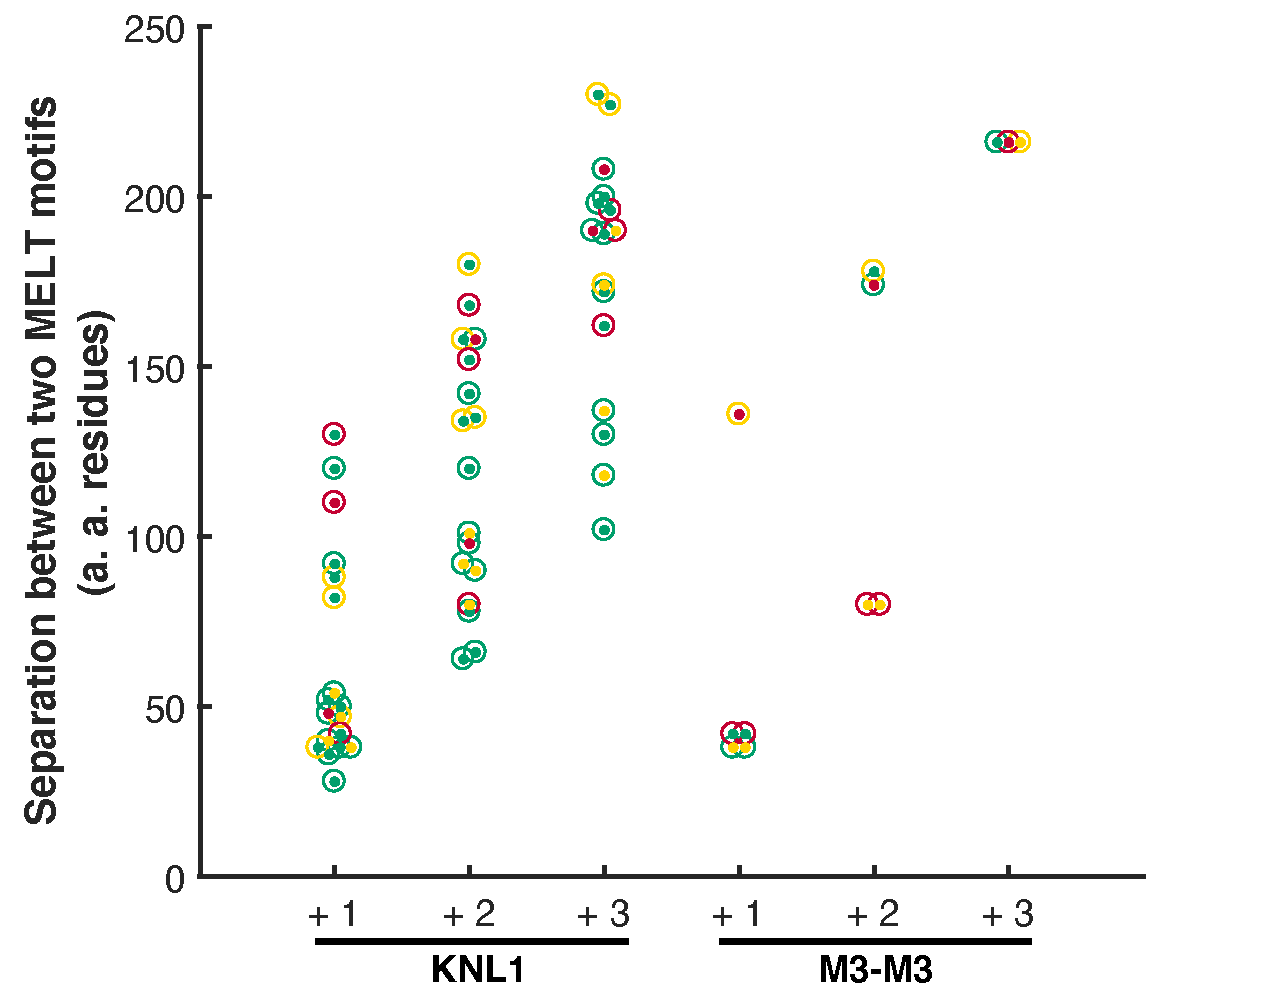
\includegraphics[width=0.6\textwidth]{chapters/figures/MELTSeparationColorCodedBeeSwarmPlot.pdf}
    \caption{\textbf{Pairwise distances between $(+1, +2, +3)$-neighboring MELT motifs in the endogenous \protein{Knl1} and the M6 (M3-M3) eSAC construct.}}
    \noindent\justifying Each ``circle \& center'' symbol represents a pair of neighboring MELT motifs. There are a total number of 19 putative MELT motifs in the endogenous \protein{Knl1} and 6 MELT motifs in the signaling scaffold of the M6 (M3-M3) eSAC construct. Therefore, we have a total number of $(18, 17, 16)$ pairs and $(5, 4, 3)$ pairs of $(+1, +2, +3)$-neighboring MELT motifs in the endogenous \protein{Knl1} and the M6 (M3-M3) eSAC construct, respectively. The coloring scheme follows the one in the original research \cite{MELTactivity} that studies the recruitment of \protein{Bub1} and is a rough estimation of the signaling activity of the corresponding MELT motifs (green: ``high'', yellow: ``intermediate'', red: ``low'').
    \label{PairwiseDistancesBetweenNeighboringMELTs}
\end{figure}

To study the effect of the distance between MELT motifs in the signaling scaffold on the SAC activity, we designed a series of eSAC assays using artificially designed signaling scaffolds [MELT\textsuperscript{12}-$1\times$linker-MELT\textsuperscript{12}, MELT\textsuperscript{12}-$2\times$linker-MELT\textsuperscript{12}, and MELT\textsuperscript{12}-$3\times$linker-MELT\textsuperscript{12}]. The total number of MELT motifs are fixed (two) and the sequence of MELT motifs adopts that of MELT\textsuperscript{12}. Various copies of the endogenous linker between MELT\textsuperscript{11} and MELT\textsuperscript{12} are inserted between the two MELT\textsuperscript{12}'s. The resulting distance between the two MELT\textsuperscript{12}'s varies from 112 to 288 \myref{DistanceEffect}, compared to a distance of 274 amino acids between the first motif and the last MELT motif in the M6 (M3-M3) construct in the previous section. From these assays, we observed that MELT\textsuperscript{12}-$3\times$linker-MELT\textsuperscript{12} has a slightly less SAC activity compared to the other two, but the difference is small and negative (about \SI{-15}{min} to \SI{-10}{min}) compared to the differences in the SAC activities between M1 and M6 (M3-M3) [as well as between M3 and M6 (M3-M3)]. Therefore, we inferred that the difference in the number of MELT motifs in the eSAC constructs is the major factor that determines its SAC activity.

\begin{figure}
    \centering
    \includegraphics[width=0.75\textwidth]{chapters/figures/DistanceEffect.pdf}
    \caption{\textbf{The distance between MELT motifs has a minor impact on the SAC activity.}}
    \noindent\justifying (A) The distance between the two MELT\textsuperscript{12} motifs in the three constructs are 112, 200, and 288 amino acids, respectively [compared to a distance of 274 amino acids between the first motif and the last MELT motif in the M6 (M3-M3) construct in the previous section]. (B-E) A summary (E) of eSAC activities of MELT\textsuperscript{12}-$1\times$linker-MELT\textsuperscript{12} (B), MELT\textsuperscript{12}-$2\times$linker-MELT\textsuperscript{12} (C), and MELT\textsuperscript{12}-$3\times$linker-MELT\textsuperscript{12} (D) as the signaling scaffold. Each gray dot represents a cell. (F) Comparison of the plateau levels of SAC response curves of the three eSAC constructs. Only cells with [eSAC activator] $> 10$ AUs are included. Data of more than 500 cells from two independent experiments were pooled for each group. The average mitotic durations are $(122.3 \pm 3.4)$, $(119.1 \pm 4.4)$, and $(108.1 \pm 5.7)$ minutes. Mean values $\pm 95\%$ confidence intervals are overlaid. Unpaired $t$-tests with Welch's correction were performed in Prism 9 (GraphPad Software).
    \label{DistanceEffect}
\end{figure}


\section{Materials and Methods}
\subsection*{Protein purification of recombinant \protein{Mps1} kinase domain from Sf9 cells}
The recombinant bacmid was generated from pCCB15 via Bac-to-Bac\textsuperscript{\textregistered} (Thermo Fisher Scientific). Baculovirus-transfected Sf9 cells (from \SI{1}{L} of culture) were pelleted down and stored at \SI{-80}{\celsius} until protein purification. Cells were resuspended in buffer IA [\SI{50}{mM} Tris-HCl (pH 7.5), \SI{300}{mM} NaCl, 0.2\% Triton X-100, \SI{20}{mM} imidazole, 0.1\% \textbeta-mercaptoethanol, and supplemented with PMSF and cOmplete\texttrademark{} EDTA-free Protease Inhibitor Cocktail (Roche) before usage] to a total volume of \SI{60}{mL}. Cells were lysed by a Dounce homogenizer (20 strokes using the loose pestle followed by 1 stroke using the tight pestle) supplied with Benzonase\textsuperscript{\textregistered} Nuclease (Sigma-Aldrich). Cell lysates were then centrifuged at \SI{18000}{rpm}, \SI{4}{\celsius} for \SI{45}{min} in a F21S-8x50y rotor. The supernatant was transferred and the pellet was discarded. \SI{5}{mL} of Ni-NTA agarose (equilibrated with buffer IA; Thermo Fisher Scientific) was added into the supernatant and the mixture was rotated at \SI{4}{\celsius} for \SI{3.5}{h}. The slurry was then washed with \SI{5}{mL} of buffer IA for 4 times. Bound proteins were eluted with buffer IB [\SI{50}{mM} Tris-HCl (pH 7.5), \SI{300}{mM} NaCl, 0.2\% Triton X-100, \SI{200}{mM} imidazole, 0.1\% \textbeta-mercaptoethanol].

\SI{2}{mL} of amylose resin was added (equilibrated with buffer IB; New England Biolabs) into eluted proteins from the Ni-NTA agarose column and the mixture was rotated at \SI{4}{\celsius} for \SI{2.5}{h}. The protein-bound amylose resin was then washed with \SI{5}{mL} of buffer IC [\SI{50}{mM} Tris-HCl (pH 7.5), \SI{300}{mM} NaCl, 0.2\% Triton X-100] for 4 times. \SI{2.5}{mL} of buffer IC followed by \SI{40}{\micro L} of \SI{1}{M} \textsc{d}-(+)-maltose stock solution was then added into the slurry. The mixture was rotated at \SI{4}{\celsius} for \SI{30}{min} and then eluted proteins were collected. The elution was loaded onto a Superdex 200 pg column (Cytiva) for size-exclusion chromatography. Fractions corresponding to the monomeric full-length 6×His-MBP-TEV-FRB*-mCherry-\protein{Mps1}\textsuperscript{kinase domain} (determined by molecular weight estimation and SDS-PAGE analysis) were subject to a subsequent Bradford protein assay (Bio-Rad Laboratories) and later used in the in vitro kinase assay.

\subsection*{Protein purification of recombinant \protein{Knl1} phosphodomain from Rosetta\texttrademark{} 2(DE3)}

pCCB9-transformed Rosetta\texttrademark{} 2(DE3) cells were induced to express 6×His-3×FLAG-TEV-MELT\textsuperscript{12-14}-mNeonGreen-2×FKBP by \SI{1}{mM} IPTG at \SI{25}{\celsius} for \SI{20}{h}. Cells from \SI{2}{L} of Luria-Bertani liquid media were harvested, resuspended in deionized water into a total volume of \SI{40}{mL}, and then stored at \SI{-80}{\celsius} until protein purification.

The cell slurry was thawed on ice and an equal volume of $2\times$ buffer A [the $1\times$ buffer A has the following composition: \SI{50}{mM} Tris-HCl (pH 7.4), \SI{500}{mM} NaCl, \SI{0.1}{mM} EDTA, \SI{0.1}{mM} EGTA, and \SI{20}{mM} imidazole] supplemented with PMSF, \SI{0.1}{mg/mL} chicken egg white lysozyme (Sigma-Aldrich), \SI{2}{mM} DTT, and cOmplete\texttrademark{} EDTA-free Protease Inhibitor Cocktail was added into the slurry. Cells were lysed by sonication for a total amount of on time of \SI{150}{s} at 62\% amplitude (Model 500 sonic dismembrator, Thermo Fisher Scientific) in a water-ice bath at \SI{0}{\celsius}. Triton X-100 was added to a final concentration of 0.5\%. Lysates were rotated for \SI{15}{min} and then centrifuged at \SI{18000}{rpm}, \SI{4}{\celsius} for \SI{45}{min} in a F21S-8x50y rotor. The supernatant was filtered through 0.45-\textmu{}m syringe filter units (MilliporeSigma) and the pellet was discarded. \SI{1.5}{mL} of Ni-NTA agarose (equilibrated with buffer A supplemented with 0.1\% Triton X-100) was added into the filtered supernatant and the mixture was rotated at \SI{4}{\celsius} for \SI{3}{h}. The slurry was then washed with \SI{10}{mL} of buffer A supplemented with 0.1\% Triton X-100 for 4 times. Bound proteins were eluted with \SI{6}{mL} of buffer B [\SI{50}{mM} Tris-HCl (pH 7.4), \SI{500}{mM} NaCl, \SI{0.1}{mM} EDTA, \SI{0.1}{mM} EGTA, 0.1\% Triton X-100, and \SI{200}{mM} imidazole] for \SI{1}{h} at \SI{4}{\celsius}. The elution was filtered through a 0.45-\textmu{}m syringe filter unit and dialyzed in a Slide-A-Lyzer\texttrademark{} dialysis cassette (10K MWCO; Thermo Fisher Scientific) overnight against an imidazole-free buffer [\SI{50}{mM} Tris-HCl (pH 7.45 at \SI{4}{\celsius}) and \SI{300}{mM} NaCl] and then loaded onto a Superdex 200 pg column for size-exclusion chromatography. Fractions corresponding to the 6×His-3×FLAG-TEV-MELT\textsuperscript{12-14}-mNeonGreen-2×FKBP (determined by molecular weight estimation and SDS-PAGE analysis) were later used in the in vitro kinase assay.

\subsection*{In vitro kinase assay using purified recombinant \protein{Mps1} kinase domain}
The substrate 6×His-3×FLAG-TEV-MELT\textsuperscript{12-14}-mNeonGreen-2×FKBP (\SI{73.1}{kDa}) was incubated with 6×His-MBP-TEV-FRB*-mCherry-\protein{Mps1}\textsuperscript{kinase domain} (\SI{124.8}{kDa}) at \SI{30}{\celsius} for \SI{5}{min} -- \SI{2}{h} in the kinase buffer [\SI{10}{mM} Tris-HCl (pH 7.5), \SI{100}{mM} NaCl, \SI{10}{mM} \ch{MgCl2}, and \SI{1}{mM} DTT] supplemented with \SI{500}{nM} rapamycin and \SI{0.25}{mM} ATP. The reactions were stopped with the Laemmli Sample Buffer (supplemented with \textbeta-mercaptoethanol, Bio-Rad Laboratories). Phosphorylation of the substrate was detected by our custom-made anti-\Peptide{MEIpTRSHTTALEC} phospho-specific rabbit polyclonal antibody (GenScript). Equal inputs of the substrate and the recombinant kinase across different groups were validated by silver staining (Bio-Rad Laboratories).
